\subsection{Machine Learning}\label{subsec:machine-learning}

\begin{frame}{Machine Learning (ML)}
    \setbeamertemplate{itemize items}[square]
    \begin{itemize}
        \item{It is computational process for improving performance based on experience.}
        \vspace{0.4cm}
        \item{ML is a subfield of Artificial Intelligence (AI) and is primarily related to Data Analysis.}
        \vspace{0.4cm}
        \item{ML approaches are commonly divided into three ($3$) broad categories:
        \setbeamertemplate{enumerate items}[circle]
        \begin{enumerate}
            \item Supervised Learning %(correct answers for each training point)
            \item Unsupervised Learning %("just make sense of the data")
            \item Reinforcement Learning %(reward sequence, no correct answers)
        \end{enumerate}}
    \end{itemize}
\end{frame}

\begin{frame}{Neural Networks (NN)}
    \setbeamertemplate{itemize items}[square]
    \begin{itemize}
        \item{A dominant class of ML algorithms.}
        \vspace{0.2cm}
        \item{ML with NN $\implies$ Deep Learning (DL)}
        \vspace{0.2cm}
        \item{Inspired by the neurophysiological experiments conducted by Hubel \& Wiesel in 1962.}
        \vspace{0.2cm}
        \item{Can approach highly complex functions and decision regions.}
        \vspace{0.2cm}
        \item[]{
        \begin{figure}[H]
            \centering
            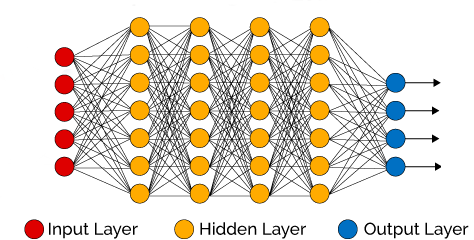
\includegraphics[width=8cm,height=3.8cm]{images/dnn.png}
            \caption{a Deep Neural Network.}
            \label{fig:dnn}
        \end{figure}}
    \end{itemize}
\end{frame}

\begin{frame}{NN learning process}
    \setbeamertemplate{itemize items}[square]
    \begin{itemize}
        \item{Assume a set $D=\{(x,y)\:|\:x\in\mathbb{R}^n,y\in\mathbb{N}\}$ of training data points.}
        \vspace{0.3cm}
        \item{A NN is a non-linear function $f$ parameterized by $w\in\mathbb{R}^d$.}
        \vspace{0.3cm}
        \item{Consider a globally continuous and differentiable \textbf{loss function} $\mathcal{L}:\mathcal{F}\times\mathcal{X}\times\mathcal{Y}\rightarrow\mathbb{R}_+$.}
        \vspace{0.3cm}
        \item{Training is performed by the mini-batch Gradient Descent (GD) algorithm
        \begin{itemize}
            \item[]{
            \begin{algorithm}[H]
                \begin{algorithmic}[1]
                    \WHILE{does not \emph{converge}}
                    \STATE \textbf{pick} randomly a mini-batch $\beta=\{(x_1,y_1),\dots,(x_{|\beta|},y_{|\beta|})\} \subset D$
                    \STATE \textbf{update} $w_{t+1}=w_t-\alpha\frac{1}{|\beta|}\sum_{i=1}^{|\beta|}\nabla_w\mathcal{L}(y_i,\hat{y_i})$
                    \ENDWHILE
                \end{algorithmic}
                \label{alg:gd}
            \end{algorithm}
            }
        \end{itemize}
        with $|\beta| \ll |D|$.}
    \end{itemize}
\end{frame}

\begin{frame}{Recurrent Neural Networks (RNN)}
    \setbeamertemplate{itemize items}[square]
    \begin{itemize}
        \item{Introduced by David Rumelhart in 1986.}
        \vspace{0.2cm}
        \item{Can handle sequential data.}
        \vspace{0.2cm}
        \item{Considers the current input and also the previously received inputs.}
        \vspace{0.2cm}
        \item{Can memorize previous inputs due to its internal memory.}
        \vspace{0.2cm}
        \item[]{
        \begin{figure}[H]
            \centering
            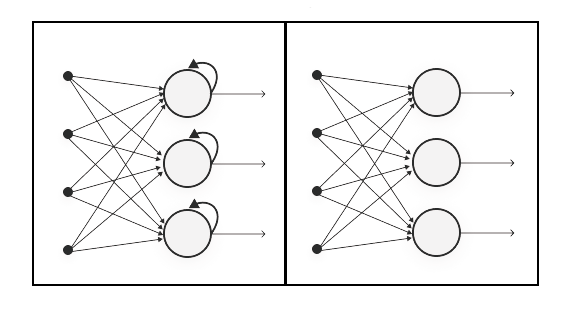
\includegraphics[width=7cm,height=3.5cm]{images/rnn-vs-fnn.png}
            \caption{a Recurrent Neural Network vs a Feed-forward one.}
            \label{fig:rnn-vs-fnn}
        \end{figure}
        }
    \end{itemize}
\end{frame}

\begin{frame}{LSTM Networks}
    \begin{columns}
        \column{0.55\textwidth}
        \setbeamertemplate{itemize items}[square]
        \begin{itemize}
            \item{LSTM for Long Short Term Memory.}
            \vspace{0.2cm}
            \item{Not fundamentally different\\from RNN.}
            \vspace{0.2cm}
            \item{Use different functions to\\compute hidden state.}
            \vspace{0.2cm}
            \item{Cells decide what to keep in memory.}
            \vspace{0.2cm}
            \item{Very effective in capturing\\long term dependencies.}
        \end{itemize}
        \column{0.45\textwidth}
        \begin{figure}
            \subfigure[\tiny{The repeating module in a standard RNN contains a single layer.}]{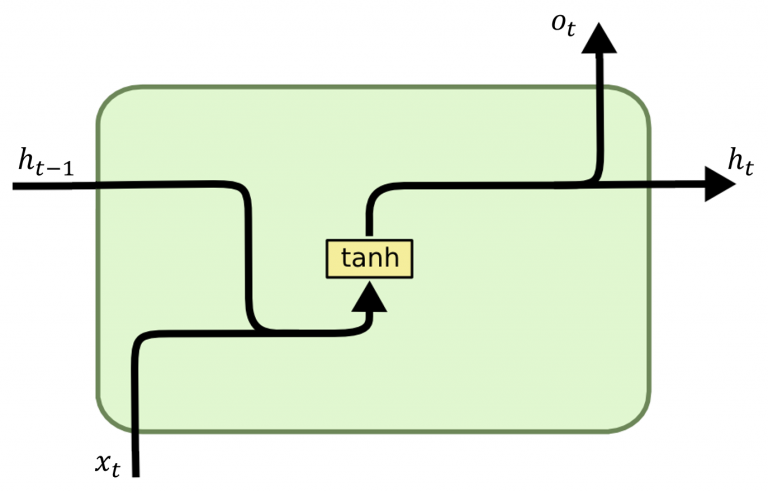
\includegraphics[width=3.8cm,height=2.5cm]{images/rnn.png}}
            \subfigure[\tiny{The repeating module in an LSTM contains four interacting layers.}]{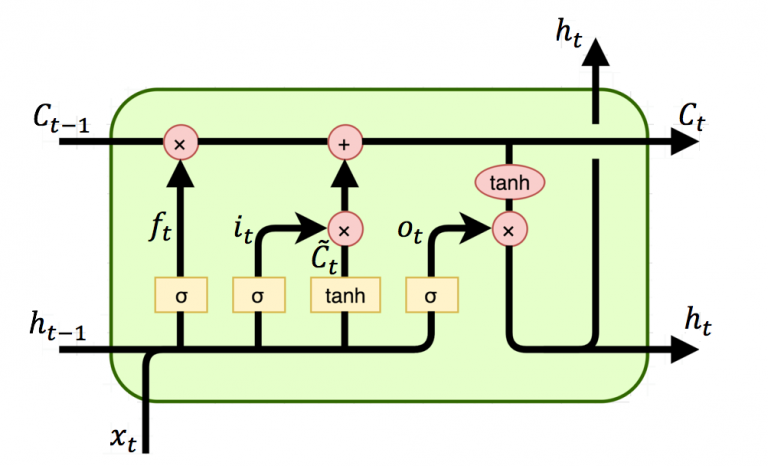
\includegraphics[width=3.8cm,height=2.5cm]{images/lstm.png}}
            \label{fig:rnn-vs-lstm}
        \end{figure}
    \end{columns}
\end{frame}

\subsection{Distributed Deep Learning}\label{subsec:distributed-deep-learning}

\begin{frame}{Network Architecture}
    \begin{columns}
        \column{0.5\textwidth}
        \setbeamertemplate{itemize items}[square]
        \begin{itemize}
            \item{A \textbf{star network} topology with
            \setbeamertemplate{itemize items}[circle]
            \begin{itemize}
                \item a \emph{parameter server}
                \item $n$ remote \emph{workers}
            \end{itemize}}
            \vspace{0.2cm}
            \item{Each worker $i \in [\,1,n]\,$ has a chunk $D_i$ of the whole training set $D$.}
            \vspace{0.2cm}
            \item{Each worker has a \textbf{replica} of the DL model.}
        \end{itemize}
        \column{0.5\textwidth}
        \begin{figure}
            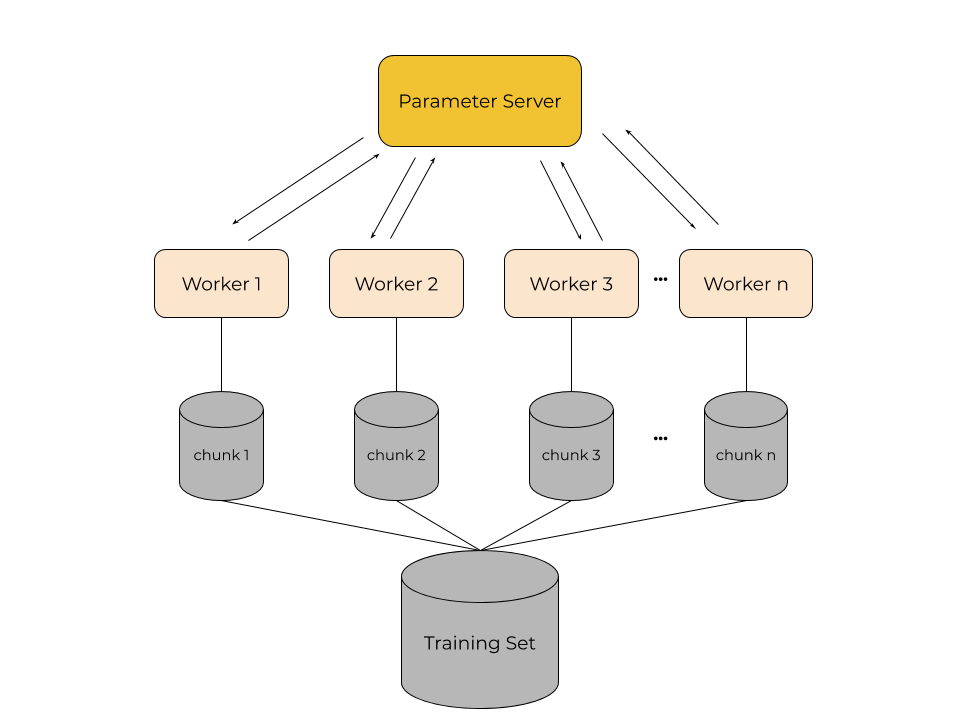
\includegraphics[width=8.5cm,height=6cm,center]{images/parameter-server.png}\label{fig:param-server}
        \end{figure}
    \end{columns}
\end{frame}

\begin{frame}{Parameter Server (PS) model}
    \setbeamertemplate{itemize items}[square]
    \begin{itemize}
        \item{The most known model for distributed DL.}
        \vspace{0.2}
        \item{\textbf{Pseudo algorithm}}
        \vspace{0.1}
        \item[]{
        \begin{algorithm}[H]
            \begin{algorithmic}[1]
                \STATE The PS initializes the parameters of the DL model.
                \STATE The PS broadcasts the model parameters to each worker.
                \STATE Each worker fits a mini-batch, taken from its chunk, using the mini-batch GD algorithm.
                \STATE When \textbf{step 3} is done, all workers send their model parameters\\to the PS where the aggregation takes place.
                \STATE While each chunk is not empty, go to \textbf{step 2}, otherwise \textbf{all done}.
            \end{algorithmic}
            \label{alg:param-server}
        \end{algorithm}
        }
    \end{itemize}
\end{frame}